\begin{flushright} {\tiny {\color{gray} basis\_p4\_2D.tex}} \end{flushright}
%~~~~~~~~~~~~~~~~~~~~~~~~~~~~~~~~~~~~~~~~~~~~~~~~~~~~~~~~~~~~~~~~~~~~~~~~~~~~~~~~~~~~~~~~~~~~~~~~~~

\begin{flushright} {\tiny {\color{gray} (tikz\_p4.tex)}} \end{flushright}
%~~~~~~~~~~~~~~~~~~~~~~~~~~~~~~~~~~~~~~~~~~~~~~~~~~~~~~~~~~~~~~~~~~~~~~~~~~~~~~~~~~~~~~~~~~~~~~~~~~

\begin{center}
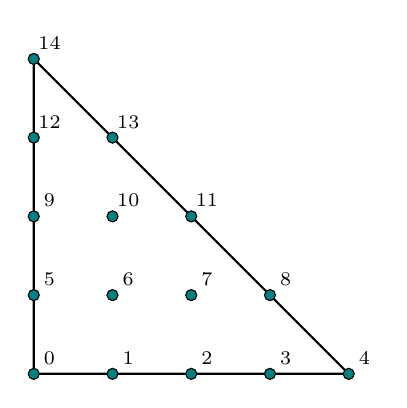
\begin{tikzpicture}
%\draw[step=0.5cm,gray,very thin] (0,0) grid (5,3.5); %bckgr grid
\draw[thick] (0,0) -- (4,0)  -- (0,4) -- cycle; 

\draw[black,fill=teal] (0,0) circle (2pt);
\draw[black,fill=teal] (1,0) circle (2pt);
\draw[black,fill=teal] (2,0) circle (2pt);
\draw[black,fill=teal] (3,0) circle (2pt);
\draw[black,fill=teal] (4,0) circle (2pt);
\draw[black,fill=teal] (0,1) circle (2pt);
\draw[black,fill=teal] (1,1) circle (2pt);
\draw[black,fill=teal] (2,1) circle (2pt);
\draw[black,fill=teal] (3,1) circle (2pt);
\draw[black,fill=teal] (0,2) circle (2pt);
\draw[black,fill=teal] (1,2) circle (2pt);
\draw[black,fill=teal] (2,2) circle (2pt);
\draw[black,fill=teal] (0,3) circle (2pt);
\draw[black,fill=teal] (1,3) circle (2pt);
\draw[black,fill=teal] (0,4) circle (2pt);

\node[] at (0.2,0.2) {\scriptsize $0$};
\node[] at (1.2,0.2) {\scriptsize $1$};
\node[] at (2.2,0.2) {\scriptsize $2$};
\node[] at (3.2,0.2) {\scriptsize $3$};
\node[] at (4.2,0.2) {\scriptsize $4$};
\node[] at (0.2,1.2) {\scriptsize $5$};
\node[] at (1.2,1.2) {\scriptsize $6$};
\node[] at (2.2,1.2) {\scriptsize $7$};
\node[] at (3.2,1.2) {\scriptsize $8$};
\node[] at (0.2,2.2) {\scriptsize $9$};
\node[] at (1.2,2.2) {\scriptsize $10$};
\node[] at (2.2,2.2) {\scriptsize $11$};
\node[] at (0.2,3.2) {\scriptsize $12$};
\node[] at (1.2,3.2) {\scriptsize $13$};
\node[] at (0.2,4.2) {\scriptsize $14$};

\end{tikzpicture}
\end{center}


The support nodes coordinates are as follows:

\begin{center}
\begin{tabular}{cccccccccccccccc}
\hline
$i\rightarrow$& 1 &2 &3 &4 &5 &6 &7 &8 &9 &10 &11 &12 &13 &14 &15 \\
\hline\hline
$r_i$&0&$\frac14$ & $\frac12$ & $\frac34$ & 1 &0 &$\frac14$&$\frac12$&
$\frac34$&0&$\frac14$&$\frac12$&0&$\frac14$&0    \\
$s_i$&0&0&0&0&0&$\frac14$&$\frac14$&$\frac14$&$\frac14$
&$\frac12$&$\frac12$&$\frac12$
&$\frac34$&$\frac34$&1\\
\hline
\end{tabular}
\end{center}

Inside the element a field $f$ is represented by a 4-th order polynomial:
\begin{eqnarray}
f^h(r,s)
&=&c_0 + c_1 r+c_2 s \nn\\
&&+ c_3 r^2 + c_4 rs + c_5 s^2 \nn\\
&&+c_6r^3 + c_7 r^2s + c_8 rs^2 + c_9 s^3 \nn\\
&&
+ c_{10} r^4 
+ c_{11} r^3s 
+ c_{12} r^2s^2
+ c_{13} rs^3
+c_{14} s^4
\end{eqnarray}

At each node the function takes a value $f_i$, $i\in[1,15]$ so that we have:
\[
\left(
\begin{array}{lllllllllllllll}
1\quad{} &0 & 0\quad{}& 0  &0&0\quad{} &0 &0&0&0\quad{} &0& 0&0&0&0\\
1 & \frac14&0&\frac{1}{16}&0&0&\frac{1}{64}&0&0&0&\frac{1}{256}&0&0&0&0 \\
1 & \frac12&0&\frac14&0&0&\frac18&0&0&0&\frac{1}{16}&0&0&0&0 \\
1 & \frac34&0&\frac{9}{16}&0&0&\frac{27}{64}&0&0&0&\frac{81}{256}&0&0&0&0 \\ 
1 &1&0&1&0&0&1&0&0&0&1&0&0&0&0 \\ \\
1 &0&\frac14&0&0&\frac{1}{16}&0&0&0&\frac{1}{64}&0&0&0&0&\frac{1}{256} \\
1 &\frac14&\frac14&\frac{1}{16}&\frac{1}{16}&\frac{1}{16}&\frac{1}{64}&\frac{1}{64}&\frac{1}{64}&\frac{1}{64}&\frac{1}{256}&\frac{1}{256}&\frac{1}{256}&\frac{1}{256}&\frac{1}{256} \\
1 &\frac12&\frac14&\frac14&\frac18&\frac{1}{16}&\frac18&\frac{1}{16}&\frac{1}{32}&\frac{1}{64}&\frac{1}{16}&\frac{1}{32}&\frac{1}{64}&\frac{1}{128}&\frac{1}{256} \\
1 &\frac34&\frac14&\frac{9}{16}&\frac{3}{16}&\frac{1}{16}&\frac{27}{64}&\frac{9}{64}&\frac{3}{64}&\frac{1}{64}&\frac{81}{256}&\frac{27}{256}&\frac{9}{256}&\frac{3}{256}&\frac{1}{256} \\
\\
1 &0&\frac12&0&0&\frac14&0&0&0&\frac18&0&0&0&0&\frac{1}{16} \\
1 &\frac14&\frac12&\frac{1}{16}&\frac{1}{8}&\frac{1}{4}&\frac{1}{64}&\frac{1}{32}&\frac{1}{16}&\frac{1}{8}&\frac{1}{256}&\frac{1}{128}&\frac{1}{64}&\frac{1}{32}&\frac{1}{16} \\
1 &\frac12&\frac12&\frac14&\frac14&\frac14&\frac{1}{8}&\frac{1}{8}&\frac{1}{8}&\frac{1}{8}&\frac{1}{16}&\frac{1}{16}&\frac{1}{16}&\frac{1}{16}&\frac{1}{16} \\ \\
1 &0&\frac34&0&0&\frac{9}{16}&0&0&0&\frac{27}{64}&0&0&0&0&\frac{81}{256} \\
1 &\frac14&\frac34&\frac{1}{16}&\frac{3}{16}&\frac{9}{16}&\frac{1}{64}&\frac{3}{64}&\frac{9}{64}&\frac{27}{64}&\frac{1}{256}&\frac{3}{256}&\frac{9}{256}&\frac{27}{256}&\frac{81}{256} \\ \\
1 &0&1&0&0&1&0&0&0&1&0&0&0&0&1 
\end{array}
\right)
\cdot
\left(
\begin{array}{c}
c_0 \\ \\
c_1 \\
c_2 \\ \\
c_3 \\
c_4 \\
c_5 \\  \\
c_6 \\
c_7 \\
c_8 \\
c_9 \\ \\
c_{10} \\ 
c_{11} \\
c_{12} \\
c_{13} \\
c_{14} 
\end{array}
\right)
=
\left(
\begin{array}{c}
f_0 \\ \\
f_1 \\
f_2 \\ \\
f_3 \\
f_4 \\
f_5 \\ \\
f_6 \\
f_7 \\
f_8 \\
f_9 \\ \\
f_{10} \\
f_{11} \\
f_{12} \\
f_{13} \\
f_{14} 
\end{array}
\right)
\]
or, 

\[
\frac{1}{256}
\left(
\begin{array}{lllllllllllllll}
256\qquad{} &0 & 0\qquad{}& 0  &0&0\qquad{} &0 &0&0&0\quad{} &0& 0&0&0&0\\
256 &64 &0&16 &0&0&4  &0&0&0&1&0&0&0&0 \\
256 &128&0&64 &0&0&32 &0&0&0&16&0&0&0&0 \\
256 &192&0&144&0&0&108&0&0&0&81&0&0&0&0 \\
256 &256&0&256&0&0&256&0&0&0&256&0&0&0&0 \\ 
\\
256 &0  &64&0&0&16& 0&0&0&4 &0&0&0&0&1\\
256 &64 &64&16&16&16& 4&4&4&4 &1&1&1&1&1\\
256 &128&64&64&32&16& 32&16&8&4 &16&8&4&2&1\\
256 &192&64&144&48&16& 108&36&12&4 &81&27&9&3&1\\
\\
256 & 0  &128&0 &0 &64& 0 & 0 & 0 & 32&0&0&0&0&16\\
256 & 64 &128&16&32&64& 4& 8 &16 &32  &1&2&4&8&16\\
256 & 128&128&64&64&64& 32&32&32&32 & 16&16&16&16&16\\
\\
256 & 0 & 192 & 0 & 0 & 144 & 0 & 0 & 0 & 108 & 0 & 0 & 0 & 0 & 81 \\ 
256 & 64 & 192 & 16 & 48 & 144 & 4 & 12 & 36 & 108 & 1 & 3 & 9 & 27 & 81
\\ \\
256 & 0 & 256 & 0 & 0 & 256 & 0 & 0 & 0 & 256 & 0&0 & 0 & 0 & 256
\end{array}
\right)
\cdot
\left(
\begin{array}{c}
c_0 \\ \\
c_1 \\
c_2 \\ \\
c_3 \\
c_4 \\
c_5 \\  \\
c_6 \\
c_7 \\
c_8 \\
c_9 \\ \\
c_{10} \\ 
c_{11} \\
c_{12} \\
c_{13} \\
c_{14} 
\end{array}
\right)
=
\left(
\begin{array}{c}
f_0 \\ \\
f_1 \\
f_2 \\ \\
f_3 \\
f_4 \\
f_5 \\ \\
f_6 \\
f_7 \\
f_8 \\
f_9 \\ \\
f_{10} \\
f_{11} \\
f_{12} \\
f_{13} \\
f_{14} 
\end{array}
\right)
\]


It is implemented in \stone~120.
See also python code in {\tt images/basis\_P4} which I wrote to test these basis functions.
